\section{Introdução}

\subsection{Padrões}
    \begin{frame}[fragile]{Definição de Padrões}
        \begin{figure}[H]
        \begin{center}
            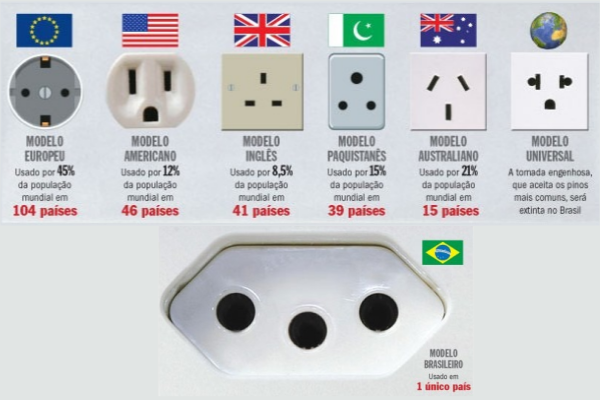
\includegraphics[scale=0.50]{images/padroes.png}
        \end{center}
        \end{figure}

        São perceptíveis \textbf{regularidades} que \textbf{repetem-se} de
        maneira \textbf{previsível} no mundo ou em um artefato produzido pelo
        homem.
    \end{frame}

    \begin{frame}[fragile]{Os Padrões no Mundo}
        \begin{figure}[H]
        \begin{center}
            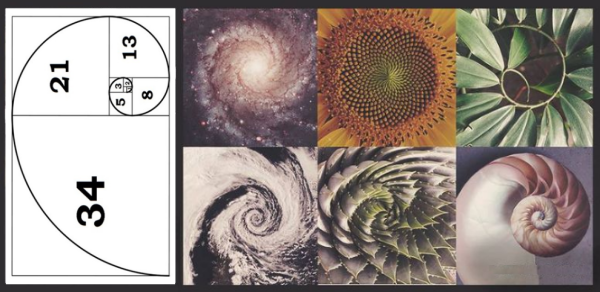
\includegraphics[scale=0.60]{images/padroes_mundo.png}
        \end{center}
        \end{figure}

        Mendes (2007) explica, em seu estudo sobre a matemática na
        \textbf{natureza}, a ocorrência da \textbf{sequência} de
        \textbf{Fibonacci} na Natureza é tão frequente que é difícil acreditar
        que é acidental \cite{mendes2007matematica}.
    \end{frame}

    \begin{frame}[fragile]{Os Padrões nos Artefatos}
        \begin{figure}[H]
        \begin{center}
            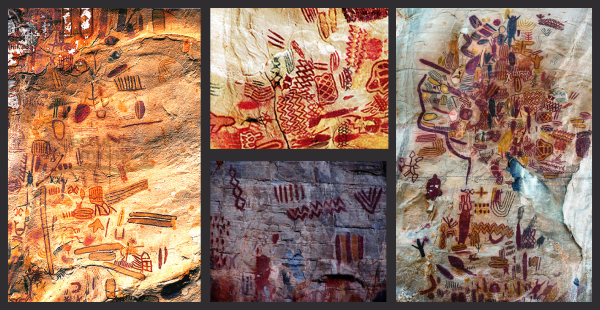
\includegraphics[scale=0.60]{images/arte_rupestre.png}
        \end{center}
        \end{figure}

        Ribeiro, L. (2007) em seu trabalho, classifica os estilos de pinturas
        rupestres do norte mineiro e sudoeste baiano
        \cite{ribeiro2007repensando}.
    \end{frame}

\subsection{Aprendizado de Máquina}
    \begin{frame}[fragile]{Aprendizado de Máquina}
        \begin{figure}[H]
        \begin{center}
            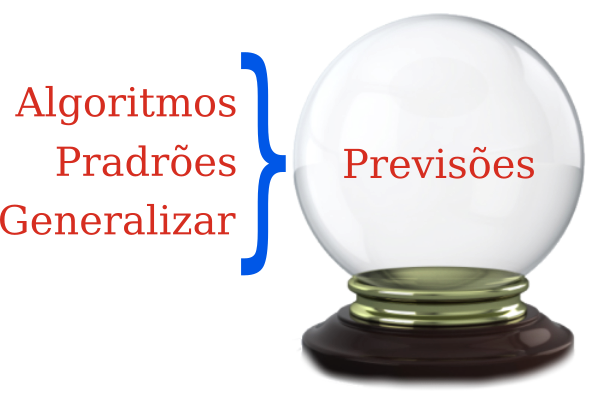
\includegraphics[scale=0.50]{images/previsao.png}
        \end{center}
        \end{figure}

        Souto, Lorena, Delbem e Carvalho explicam, o Aprendizado de Máquina,
        provê técnicas capazes de aprender automaticamente a partir dos dados
        disponíveis e produzir hipóteses úteis \cite{de2003tecnicas}.

  \end{frame}

  \begin{frame}[fragile]{Aprendizado de Máquina}

    \centering
    Qual é a \textbf{classe} da sétima linha?

    \begin{table}[]
    \centering
    \begin{tabular}{l|c|c|c|c|c|}
    \cline{2-6}
                            & \textbf{Cores}           & \textbf{R}   & \textbf{G}   & \textbf{B}   & \textbf{Classe} \\ \hline
    \multicolumn{1}{|l|}{1} & \cellcolor[HTML]{FF0000} & \textit{255} & \textit{0}   & \textit{0}   & Quente          \\ \hline
    \multicolumn{1}{|l|}{2} & \cellcolor[HTML]{0000FF} & \textit{0}   & \textit{0}   & \textit{255} & Quente          \\ \hline
    \multicolumn{1}{|l|}{3} & \cellcolor[HTML]{00FF00} & \textit{0}   & \textit{255} & \textit{0}   & Quente          \\ \hline
    \multicolumn{1}{|l|}{4} & \cellcolor[HTML]{FAEBD7} & \textit{250} & \textit{235} & \textit{215} & Fria            \\ \hline
    \multicolumn{1}{|l|}{5} & \cellcolor[HTML]{EEEEE0} & \textit{238} & \textit{238} & \textit{224} & Fria            \\ \hline
    \multicolumn{1}{|l|}{6} & \cellcolor[HTML]{E0EEEE} & \textit{224} & \textit{238} & \textit{238} & Fria            \\ \hline
    \multicolumn{1}{|l|}{7} & \cellcolor[HTML]{8B2252} & \textit{139} & \textit{34}  & \textit{82}  & \textbf{???}               \\ \hline
    \end{tabular}
    % \caption{Encontre um padrão e classifique a cor.}
    \label{my-label}
    \end{table}
  \end{frame}

  \begin{frame}[fragile]{Aprendizado de Máquina}
    \centering
    Encontrar \textbf{padrões}, \textbf{generalizar} e \textbf{predizer}!
    \begin{table}[]
    \centering
    % \caption{My caption}
    \label{my-label}
    \begin{tabular}{l|c|c|c|c|c|c|c|}
    \cline{2-7}
                            & \textbf{Cores}           & \textbf{R}   & \textbf{G}   & \textbf{B}   & \multicolumn{1}{l|}{\textbf{Soma(RGB)}} & \textbf{Classe} \\ \hline
    \multicolumn{1}{|l|}{1} & \cellcolor[HTML]{FF0000} & \textit{255} & \textit{0}   & \textit{0}   & \textit{255}                       & Quente          \\ \hline
    \multicolumn{1}{|l|}{2} & \cellcolor[HTML]{0000FF} & \textit{0}   & \textit{0}   & \textit{255} & \textit{255}                       & Quente          \\ \hline
    \multicolumn{1}{|l|}{3} & \cellcolor[HTML]{00FF00} & \textit{0}   & \textit{255} & \textit{0}   & \textit{255}                       & Quente          \\ \hline
    \multicolumn{1}{|l|}{4} & \cellcolor[HTML]{FAEBD7} & \textit{250} & \textit{235} & \textit{215} & \textit{700}                       & Fria            \\ \hline
    \multicolumn{1}{|l|}{5} & \cellcolor[HTML]{EEEEE0} & \textit{238} & \textit{238} & \textit{224} & \textit{700}                       & Fria            \\ \hline
    \multicolumn{1}{|l|}{6} & \cellcolor[HTML]{E0EEEE} & \textit{224} & \textit{238} & \textit{238} & \textit{700}                       & Fria            \\ \hline
    \multicolumn{1}{|l|}{7} & \cellcolor[HTML]{8B2252} & \textit{139} & \textit{34}  & \textit{82}  & \textit{255}                       & \textbf{Quente}          \\ \hline
    \end{tabular}
    \end{table}
  \end{frame}

\subsection{Problema de Pesquisa}
  \begin{frame}[fragile]{Problema de Pesquisa}
    \begin{figure}[H]
    \begin{center}
        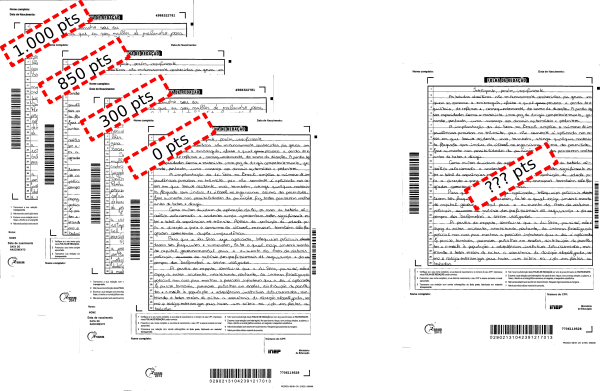
\includegraphics[scale=0.50]{images/problema_pesquisa.png}
    \end{center}
    \end{figure}

    Dado um \textit{corpus} de redações rotuladas, é possível \textbf{recuperar padrões}
    implícitos nos textos e \textbf{valorar} uma \textbf{nova amostra}?
  \end{frame}